\subsection{Construtor}

Como visto anteriormente através de exemplos utilizando linguagem de
programação \acs{PHP}, os objetos são criados (instanciados) utilizando-se um
operador especial, este operador chama-se \textit{new}.


Na Figura \ref{fig:metodoConstrutor}, tem-se um exemplo de método construtor
utilizando a linguagem \acs{PHP}:

\begin{figure}[h!tb]
	\caption{Método construtor implementado na linguagem PHP}
	\label{fig:metodoConstrutor}

	\centering
	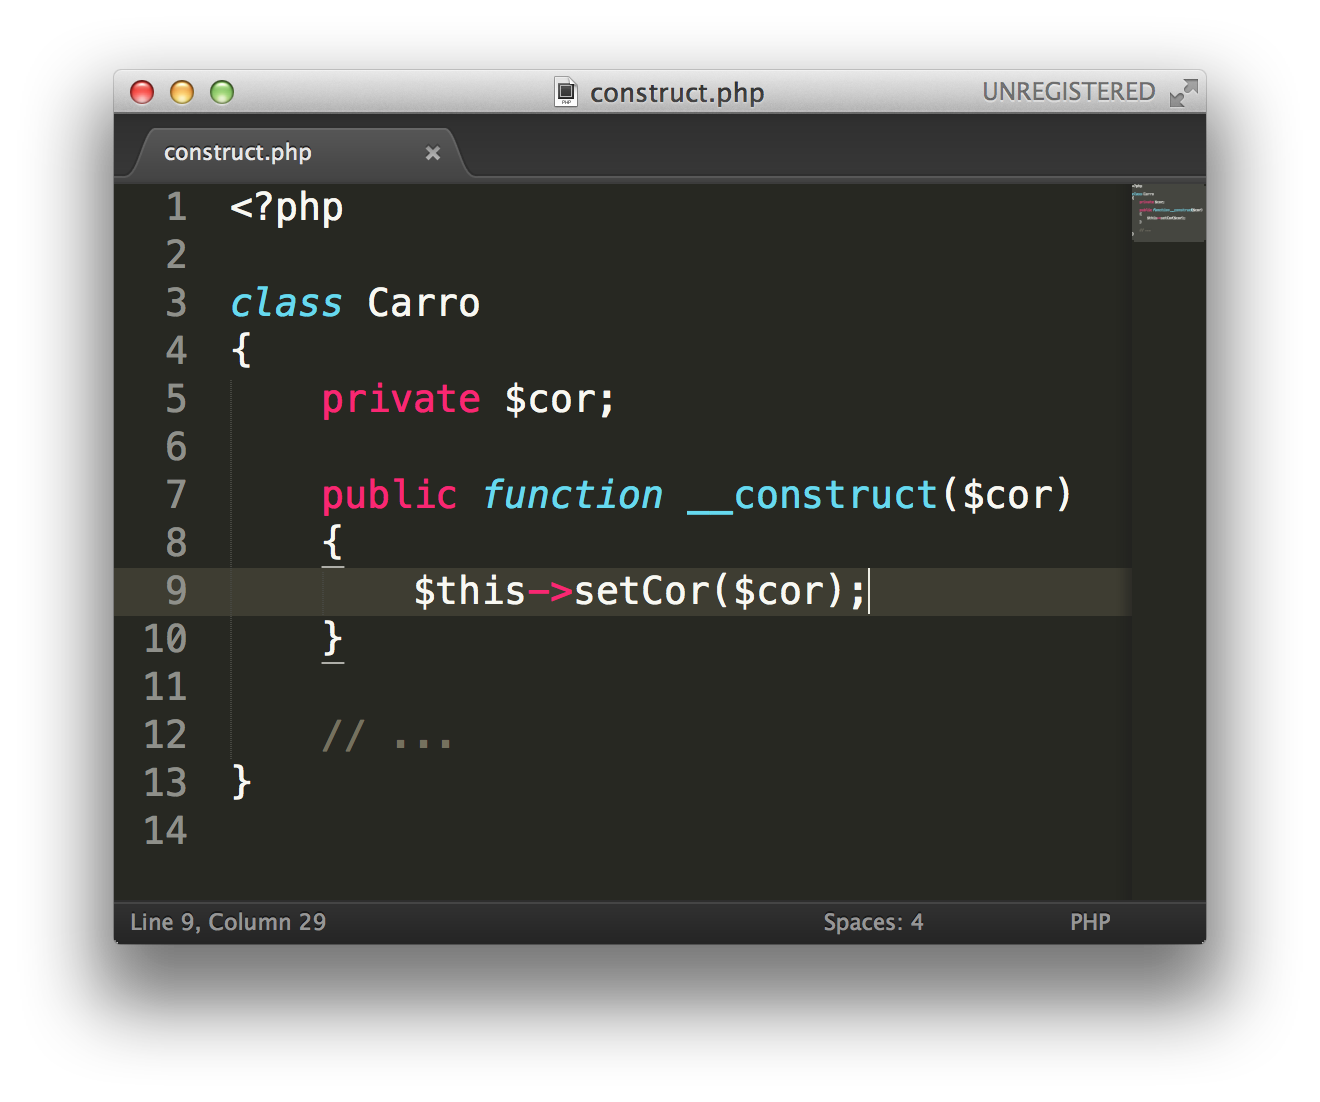
\includegraphics[width=0.75\textwidth]{images/construct.png}

	\centering
	\footnotesize Fonte: \fonteOAutor
\end{figure}

\FloatBarrier 	% Este comando impede que as imagens
				% flutuem a partir deste ponto no seu documento

A seguir, é apresentado em detalhes as linhas de código exibidas na Figura 
\ref{fig:metodoConstrutor}:

\begin{enumerate}[a)]
    \item linha 1: vê-se o início da execução de um bloco de código PHP;
    \item linha 5: define-se a propriedade \textbf{\$cor};
    \item linha 7: identifica-se o método construtor, sendo que, recebe como
    parametro a cor de um veículo;
    \item linha 9: atribuí-se o valor informado durante a instanciação da classe
    \textit{Carro} através do método \textit{setCor}.
\end{enumerate}

Segundo \citeonline{learningJava}, um construtor é um método especial que tem
como responsabilidade inicializar as propriedades de uma classe. Sendo que,
diferentemente de outras linguagens, como por exemplo Java que nomeia o  método
construtor com o mesmo nome da classe, a linguagem de script \acs{PHP} define que um
método construtor deve chamar-se \textit{\_\_construct}.

Sabendo disto, toda vez que o interpretador encontrar a palavra reservada
\textit{new} este irá executar o método construtor da classe que está sendo
instanciada.

Caso você defina uma classe e não informe explicitamente um método construtor, a
linguagem em tempo de execução irá inicializar as propriedades com valores nulos.

Além disto, os métodos construtores - da mesma forma que métodos convencionais –
podem aceitar parâmetros de inicialização \cite{learningJava}.

Como foi visto anteriormente, os métodos construtores são peças-chave para
permitir a configuração inicial de um objeto, na sequência, será apresentado o conceito referente a
métodos destrutores.
